\documentclass[a4paper,10pt]{article}
\usepackage[utf8x]{inputenc}
%\usepackage[utf8]{inputenc}
\usepackage{graphicx}
\usepackage{color}
\usepackage[table]{xcolor}
\usepackage{url}
\usepackage{enumitem}% http://ctan.org/pkg/enumitem
%\usepackage{algorithm, algorithmicx}
\usepackage[noend]{algpseudocode}
\usepackage{comment}
\usepackage[standard]{ntheorem}
\usepackage{multirow}
\usepackage{subcaption}
\usepackage{caption}
\usepackage[noadjust]{cite}
\usepackage{pdflscape}
\usepackage{lipsum}
\usepackage{capt-of}
\usepackage[linesnumbered,ruled,vlined]{algorithm2e}
\usepackage{amsmath,amssymb,amsfonts}
\usepackage{threeparttable}

\newtheorem{notation}{Notation}


\setlength{\textheight}{9.2in}
\setlength{\textwidth}{6.4in}

\setlength{\oddsidemargin}{0mm}
\setlength{\evensidemargin}{0mm}
\setlength{\topmargin}{-0.3in}

\newcommand{\sat}{$\;\triangleleft\;$}
\newcommand{\nsat}{$\;\ntriangleleft\;$}

\newcommand{\subgraphname}{part}
\newcommand{\subgraphnamespace}{part }
\newcommand{\subgraphnameCaps}{Part}

\usepackage[bookmarks=false]{hyperref}
\hypersetup{
	colorlinks,
	citecolor=black,
	filecolor=black,
	linkcolor=black,
	urlcolor=black
}
\graphicspath{{./images/}{./results/}}
\newcommand{\numBytesOffChip}{\mathbb{B}}
\newcommand{\numOverlap}{\delta}
\newcommand{\busWidth}{BW}
\newcommand{\dataWidth}{DW}
\newcommand{\dataLength}{l}
\newcommand{\addressSym}{Addr}
\newcommand{\BuffSize}{buffSize}
%\newcommand{\EXPANDER}{{\scriptsize  {EXPANDER}}\xspace}

\begin{document}
	
\begin{titlepage}
	
	\begin{center}
		
		\vspace{4cm}
		\LARGE \textbf{A FRAMEWORK FOR MAPPING NEURAL NETWORKS ON PARALLEL ARCHITECTURES}\\
		
		\vspace{2cm}
		
		\large {A synopsis submitted in partial fulfillment of the requirements for the degree\ \\}
		\vspace{0.5cm}
		\large {of\ \\}
		\vspace{0.5cm}
		\Large \textbf{Doctor of Philosophy \ \\}
		\vspace{0.5cm}
		
		\large \ \\ \ \\ Submitted by: \ \\
		\Large \textbf{SAURABH TEWARI \ \\ (2015CSZ8046)} 
		
		\large {\ \\ under the guidance of \ \\}
		% \vspace{0.2cm}
		\large \textbf{ Prof. Anshul Kumar\\ }
		\large \textbf{ Prof. Kolin Paul\\ }
		% \large {Department of Computer Science and Engineering \ \\}
		\vspace{2.0cm}
		\hspace{0cm}
		
\includegraphics[scale=1.0]{images/logo.pdf} \\
		\vspace{2.0cm} 
		\Large {DEPARTMENT OF COMPUTER SCIENCE \& ENGINEERING}\\
		\Large {INDIAN INSTITUTE OF TECHNOLOGY DELHI \\ NEW DELHI}\\
		% \vspace{2cm}
	\end{center}
	
\end{titlepage}
\pagenumbering{roman}
\section*{List of Included Papers}
This thesis is based on the following publications:

\textbf{Published:}

\newcounter{saveenum}

\begin{enumerate}
\item \textbf{S. Tewari}, A. Kumar and K. Paul, ``\textit{SACC: Split and Combine Approach to Reduce the Off-chip Memory Accesses of LSTM Accelerators}'', in DATE 2021.

\item \textbf{S. Tewari}, A. Kumar and K. Paul, ``\textit{Minimizing Off-Chip Memory Access for CNN Accelerators}'', in IEEE Consumer Electronics Magazine 2021.

\item \textbf{S. Tewari}, A. Kumar and K. Paul, ``\textit{Bus Width Aware Off-Chip Memory Access Minimization for CNN Accelerators}", in ISVLSI 2020.

\item D. Stathis, Y. Yang, \textbf{S. Tewari}, A. Hemani, K. Paul, M. Grabherr and R. Ahmad, ``\textit{Approximate Computing Applied to Bacterial Genome Identification using Self-Organizing Maps}'', in ISVLSI 2019.

\setcounter{saveenum}{\value{enumi}}
\end{enumerate}



%\textbf{In-review/Under preparation:}
%\begin{enumerate}
%  \setcounter{enumi}{\value{saveenum}}
%
%\item \textbf{Rajesh Kedia}, Shikha Goel, M. Balakrishnan, Kolin Paul, and Rijurekha Sen. ``\textit{Design space exploration of FPGA based system with heterogeneous DNN accelerators}''. Submitted to IEEE Embedded Systems Letters.
%
%\item \textbf{Rajesh Kedia}, M. Balakrishnan, and Kolin Paul. ``\textit{An integrated flow for designing Context-aware Adaptive Embedded Systems}'' -- under preparation.
%
%\item Shikha Goel, \textbf{Rajesh Kedia}, M. Balakrishnan, and Rijurekha Sen. ``\textit{INFER: INterFerence-aware Estimation of Runtime for concurrent DNN execution on DPUs}'' -- under preparation.
%
%\end{enumerate}




\newpage
\setcounter{tocdepth}{2}
\tableofcontents
\newpage

\pagenumbering{arabic}
\begin{comment}
	1. Introduction - 2 pages
	2. Related work - 0.5 pages
	3. Overall flow - 0.75 pages
	4. Graphical representation - 2 pages
	5. DSE flow - 2 pages
	6. Runtime controller generation - 1.5 page
	7. Case studies - 3.5 pages
	a. RBD - (0.5 page)
	b. MAVI - (2 pages)
	c. DPU - (1 page)
	8. Conclusion - 0.5 page
	9. References - 2 pages
\end{comment}
\section{Introduction}

\subsection{Why Off-Chip Memory Access Optimization}
\subsubsection{Impact on performance}
DNN accelerators have large number of processing elements (PEs) to exploit the parallelism of DNNs. While these PEs can perform several operations per cycle, their performance is limited by off-chip memory bandwidth. In the near forseeable future, off-chip memory accesses limits the system performance~\cite{williams2009roofline}. Fig.~\ref{fig:roofline} shows, two kernels with different compute intensity (FLOPS/byte), possibly due to different data reuse techniques. Kernel 2 can perform more computations per byte, compared to Kernel 1. Performance of Kernel 2 is limited by computational roof and it utilizes the compute resources fully (compute bound), while Kernel 1's performance is limited by memory bandwidth (memory bound).
\begin{figure}[!htb]
	\centering
	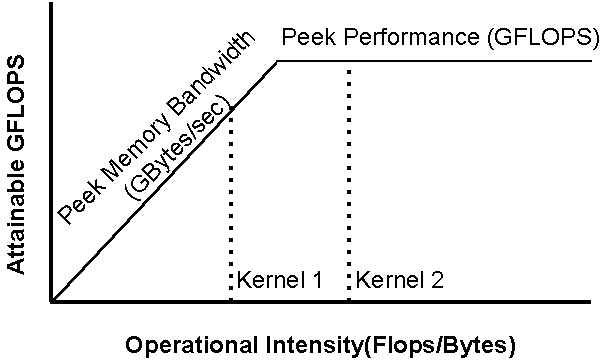
\includegraphics[width=0.6\linewidth]{./images/roofline}
	\caption{roofline model}
	\label{fig:roofline}
\end{figure}
Memory bound kernels results in under-utilization of compute resources, which results in degraded performance and energy consumption. To improve the DNN accelerators' performance, maximizing the data reuse from on-chip memories is essential.
\subsubsection{Impact on Energy Consumption}
The energy of DNN accelerators is the sum of computations and data accesses energy. 
\begin{equation}
	E=E_{comp} + E_{data}
\end{equation}
$E_{comp}$ for a DNN layer depends on the number of operations in the layer, which is fixed as it depends on layer shape e.g. number of activations, filters, and filter sizes. However $E_{data}$ can be optimized using data reuse techniques. Operations of CNN involve three kinds of data and $E_{data}$ is the sum of energies for accessing all three data types.
\begin{align}
	E_{data}&=E_{ifm}+E_{ofm}+E_{wts} \\
	E_{i}&=V_{i}*R_{i}*DW
\end{align}
where $i\in \{ifm,ofm,wts\}$ and $DW$ is the data width. A typical DNN accelerator system has multiple levels of memory hierarchy. Each level of memory has different size, energy and access time. The off-chip memory (DDR) has the largest size, and highest energy and access cost compared to other levels of memories in hierarchy.  

The off-chip memory access energy is upto two orders higher compared to on-chip memory access energy. Figure~\ref{fig:dataAccessEnergy} illustrates the impact of data reuse from on-chip memories. 
\begin{figure}[!htb]
	\centering
	\subfloat[no reuse]
	{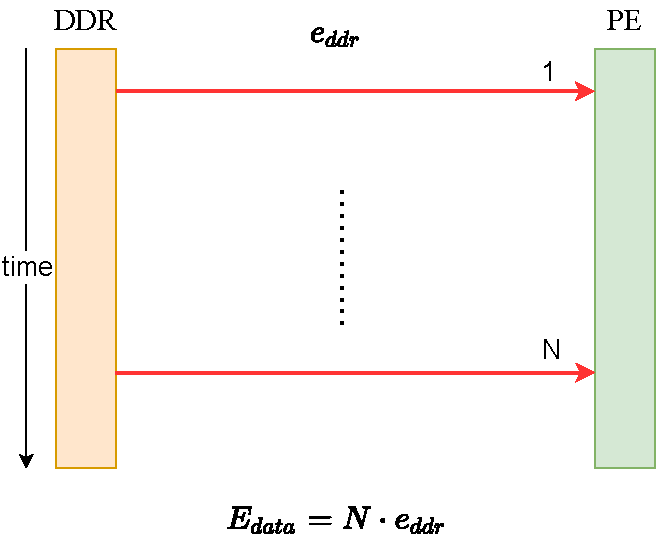
\includegraphics[width=0.4\textwidth]{energyDDR_noreuse.pdf}
		\label{fig:energyNoReuse}}
	\hfil
	\subfloat[reuse ($\times{n}$) from on-chip memory L1]
	{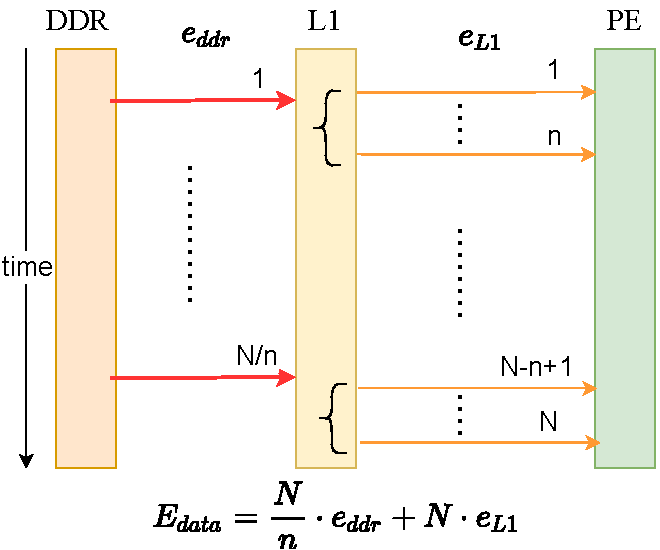
\includegraphics[width=.4\textwidth]{energy_reuse.pdf}
		\label{fig:energy_reuse}}
	\caption{data access energy $E_{data}$ with and without reuse.}
	\label{fig:dataAccessEnergy}
	\vspace{-1.0em}	
\end{figure}
The energy efficiency of an accelerator system with 2 levels of memory (DDR and L1) can be computed as below,
\begin{align*}
	\text{energy-efficiency} &= (1-\frac{E^2_{data}}{E^1_{data}})\times{100}\\
	&= (1-(\frac{1}{n}+\frac{e_{L1}}{e_{ddr}}))\times{100}
\end{align*}
As, $e_{L1} << e_{DDR}$, the ratio $\frac{e_{L1}}{e_{ddr}}$ is very small and the energy efficiency depends on number of reuses ($n$) from on-chip memory $L1$. It improves considerably with increasing the number of data reuse ($n$). 

In this work, we focus on the key issue to improve the performance and energy efficiency of DNN accelerators by reducing the off-chip memory accesses and maximizing the data reuse from on-chip memories.

\section{About the Framework}
It is arduous to create a generic framework for large variety of DNNs and accelerator architectures. However, most of the modern DNNs and accelerator's architectures share similar architectural and algorithmic features. Therefore, we propose a mapping framework that addresses the most challenging problems faced by modern DNN accelerators and that are applicable to most of these DNNs accelerators.
\begin{enumerate}
	\item Inferencing or usage of DNNs are frequently performed on edge devices. These edge devices  are resource constraints and usually battery operated. They have tight energy budget which motivates to optimize the energy consumption of these DNN on edge devices. Secondly, the short response time is also expected to improve the user experience.
   \item To optimize the performance of DNN based applications, DNN accelerators are commonly used. These accelerators have several compute units to perform large number of computations in parallel to improve the performance and user response time. However energy efficiency of these accelerators is far from desired, which restricts their usage in edge devices.
   \item DNNs have large amount of parallelism, which can be exploited to speed up the processing, however limited memory bandwidth is the bottleneck. 
   \item It is observed, that more than 80\% of overall energy consumption is due to off-chip memory accesses. Hence optimizing the off-chip memory accesses is the key to improve the energy efficiency of these DNN accelerators.
\end{enumerate}
\begin{figure}[ht]
	\centering
	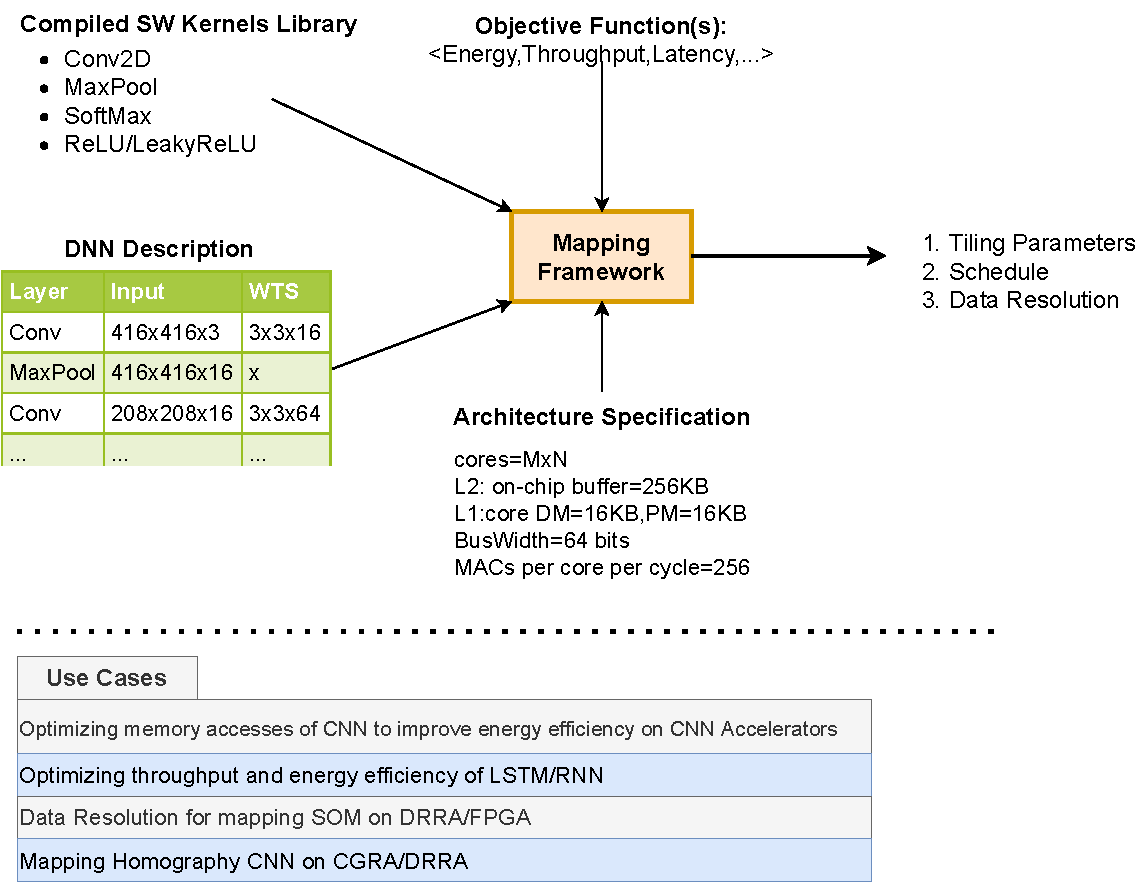
\includegraphics[width=\linewidth]{./images/blockDiagram}
	\caption{Mapping DNN on coarse grain parallel architectures}
	\label{fig:introduction}
\end{figure}
Our main contributions in this thesis dessertations are
\begin{enumerate}
	\item  We identify the key issue to be addressed for DNN accelerator's wide usage in energy constraint devices is their off-chip memory accesses. We propose a mapping framework which takes input DNNs shape and sizes and analyzes the performance and energy consumption of DNN accelerators while considering accelerator's architectural parameters.
	\item We propose a model that precisely estimates the off-chip memory accesses and the energy consumption of the DNN's layers, while taking into account the accelerator's architectural parameters.
	\item We propose an approach that determines the optimal partitoning of the DNN layers for reducing the off-chip memory accesses and energy consumptions. We analytically express the off-chip memory accesses of DNNs  using the layer shapes and tiling parameters and express it as a constraint optimization problem.
	\item We propose a novel data reuse approach to improve the run time, energy efficiency of recurrent neural networks (RNN). The proposed approach schedules the computations in a way that reduces the memory accesses of large matrices by half and optimizes the performance and energy efficiency of RNN accelerators.
	\item We analyzed the impact of data bit width on the performance, energy consumption and the accuracy of neural networks. We experimented with different data bit widths to analyze the trade-off between accuracy and energy efficiency of the NNs on reconfigurable parallel architectures.
\end{enumerate}

\subsection{Related Work}
We compare our approaches and show that our work significantly improves the performance and energy efficiency of DNN accelerators compared to the state of the art. To address the computational and energy efficiency of DNNs, several ASIC~\cite{conti2018chipmunk,wang2017accelerating,azari2020elsa} and FPGA based accelerators~\cite{chang2015recurrent,ferreira2016fpga,lee2016fpga,guan2017fpga,han2017ese} are proposed. The energy efficiency of DNN accelerators is critical for their widespread usage, and off-chip memory access is the key to improving energy consumption. Most of these works focused on improving energy efficiency by reducing off-chip memory accesses. Figure~\ref{fig:dataEnergyRelatedWork} shows broad categories of state of the art approaches that aim to improve energy efficiency of DNN accelerators by reducing the off-chip memory accesses.
\begin{figure}[!htb]
	\centering
	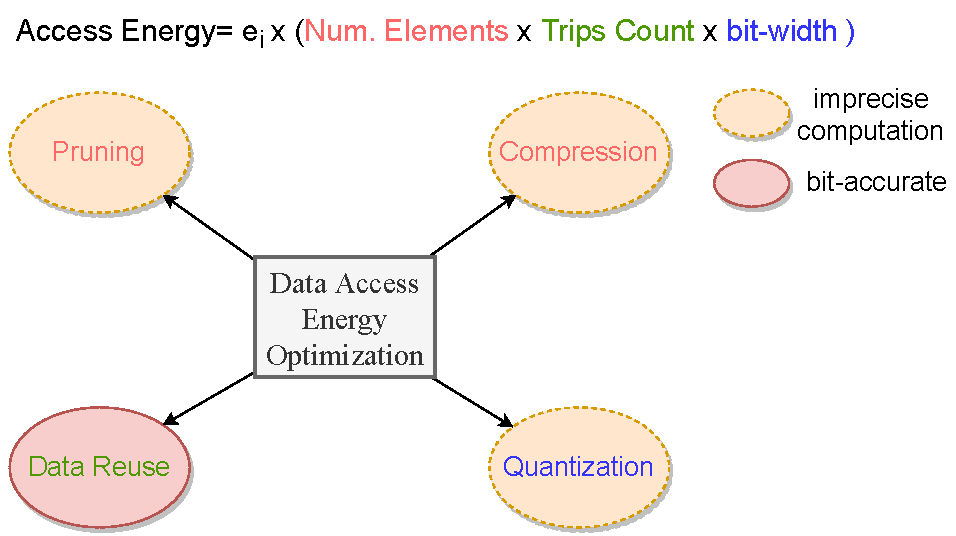
\includegraphics[width=0.4\textwidth]{./images/dataEnergyOptRelatedWork}
	\caption{Energy efficiency optimization approaches}
	\label{fig:dataEnergyRelatedWork}
\end{figure}
Some approaches~\cite{lee2016fpga, rybalkin2018finn, ferreira2016fpga} used on-chip memory to store all the weights. Sizes of weights in recent multi-layer LSTM models can be several MB's, and using large on-chip memory is expensive. These approaches are not scalable and effective only for small LSTM models. The proposed approach is independent of model size and effective for large LSTM models.

Several approaches used the fact that neural networks are error-tolerant and have lots of redundancy. They used the quantization and pruning techniques to compress the models' size. Approaches~\cite{ferreira2016fpga,wang2018c} used 18-bit, Chang et al.~\cite{chang2015recurrent} used 16-bit, Han et al.~\cite{han2017ese} used 12-bits precision for storing the inputs and weights, Lee et al.~\cite{lee2016fpga} used 8-bit inputs and 6-bits for weights to reduce the model size. The proposed approach is orthogonal to the quantization techniques and can be integrated with different quantization techniques to reduce the memory accesses further. 

Han et al.~\cite{han2017ese} used pruning to compress the model. However, pruning results in irregular network structure, and the sparse matrix require additional computational and storage resources and causes unbalanced load distribution. To overcome this Wang et al.~\cite{wang2018c} used block-circulant matrices representations to compress the LSTM/RNN model and to eliminate irregularities resulted from compression. Some approaches (\cite{park2019balancing,han2017ese,park2018maximizing}) used load balance aware pruning techniques to overcome the unbalanced load distribution problem. Quantization and pruning approaches impacts the accuracy of the networks and may not be suitable where accuracy is at priority. 

The other line of works reduced the memory accesses without compromising the accuracy of the network by applying the data-reuse techniques. Que et al.~\cite{que2019efficient} proposed a blocking-batching scheme to reuse the LSTM weights fetched from external memory. Their approach reuses the weights of $W$ matrix on a group of input vectors, by processing those input vectors as a batch. The input vectors in the same batch share the same weight matrices ($W$). However, it is difficult to collect required number of input vectors. As the LSTM cell states computations depend on cell states of the previous time-step, benefit of their batching schemes is limited to $W$ matrix. Reusing weights of $R$ across different time-steps has not been successful because of the state dependency.

Park et al.(~\cite{park2020time}) proposed a time step interleaved weight reuse scheme (TSI-WR) which reuses the weights of $R$ matrix between two adjacent time steps by performing computations in a time-interleaved manner. Their approach logically partitions the $R$ matrix into blocks. A block is accessed from off-chip memory to compute the two consecutive hidden state vectors partially. However, their approach do not fully exploit the data reuse, and several weights are accessed repeatedly from the off-chip memory. In addition, the data reuse in TSI-WR approach depends on the on-chip storage size which limits the benefits of their approach.

\section{The Mapping Framework}
The mapping framework optimizes the performance of feed-forward and recurrent neural networks. Each of these networks has specific challenges that are addressed differently. 
\subsection{Off-chip Memory Access Estimation Model}\label{sec:OffChipAccessModel}
DNNs have large amount of parallel operations. However due to large volume of data required for performing the parallel operations, the DNN acclerators' performance are limited by memory bandwidth. In addition, the DNN accelerators have limited on-chip memory, which constrains the data size that can be stored in on-chip memory. The off-chip memory accesses of a layer depends significantly on the tile dimensions~\cite{zhang2015optimizing, Li2018SmartShuttleOO}. Determining optimal tile dimensions requires analyzing off-chip memory accesses for different tile dimensions. Memory accesses also depend on the data bit width and architectural parameters of the accelerator like bus width. 

The CNN accelerators use a wide data bus to access off-chip memory to meet the high memory bandwidth requirement~\cite{Chen2016EyerissAS,chen2014diannao}. If the number of bytes accessed from an off-chip memory address is not a multiple of bus width or the address is not aligned to the word boundary, it results in unused bytes lanes of the data bus. Figure~\ref{fig:AXI_AccesseOn64BitDataBus} shows examples of memory accesses on a 64-bit data bus.  Fig.~\ref{fig:AXI_AccesseOn64BitDataBus}a shows a read transaction of 8 bytes from an aligned address and uses the full bus width. However, if only 5 bytes are read from an aligned address, as shown in \figurename~\ref{fig:AXI_AccesseOn64BitDataBus}b, 8 bytes are still accessed. If 5 bytes are read from an unaligned address, it results in 16 bytes of data access, as shown in Fig.~\ref{fig:AXI_AccesseOn64BitDataBus}d. The unused byte lanes do not carry any useful data, but they contribute to overall energy consumption. The length of the data read should be chosen such that bus utilization is high, and off-chip memory accesses and energy consumption are minimized.
\begin{figure}[!htb]
	\centering
	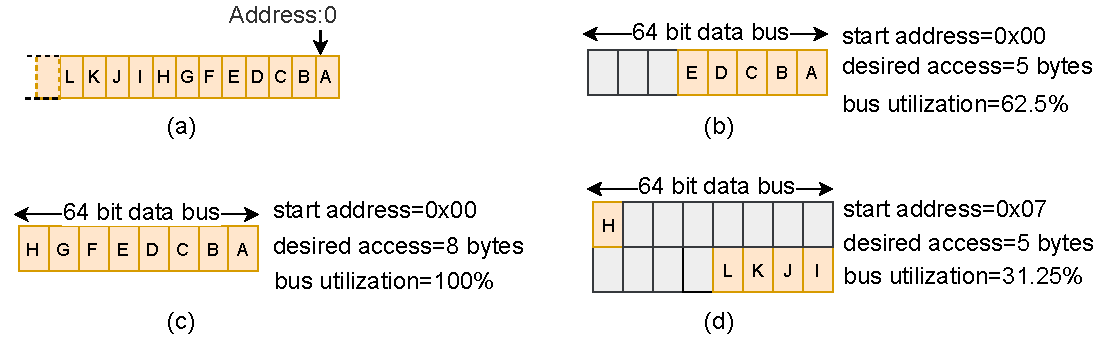
\includegraphics[width=0.7\textwidth]{./images/BurstTranscationOnAXI}
	\caption{Off-chip memory accesses on 64-bit wide data bus}
	\label{fig:AXI_AccesseOn64BitDataBus}
\end{figure}
To estimate the performance and energy efficiency, we have developed an offline model that estimates the off-chip memory accesses while taking into account the data alignment and memory bus width.

\subsection{Optimal data partitioning for CNNs}
Due to limited on-chip memory and large layer data sizes, the CNN accelerators apply loop tiling to partition the layer data. Loop tiling is a compiler  technique~\cite{aho2006compilers} that partitions the loop iteration space and large arrays into smaller tiles to increase the data locality and ensures that data fits into smaller memories. 

Fig.~\ref{fig:partitioningDataUsingTiling} shows a CL data stored in off-chip memory and its tiles in the accelerator's on-chip buffer.
\begin{figure}[!htb]
	\centering
	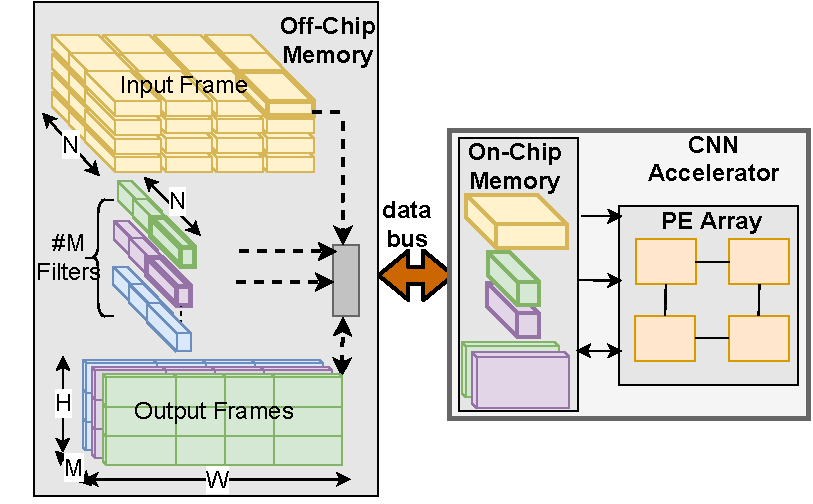
\includegraphics[width=0.5\textwidth]{images/AboutTheCNNTiles.pdf}
	\caption{CNN layer tiles in off-chip and on-chip memory}
	\label{fig:partitioningDataUsingTiling}
	\vspace{-1.0em}
\end{figure}
For a given data reuse scheme, all the tiles of a 3D data make the same number of trips from off-chip memory. The off-chip memory access of 3D data can be computed as following
\begin{align}\label{eq:BasicOffChip3DDataAccess}
	\numBytesOffChip_{3D}{=}r{\times} \sum_{t=1}^{N_{tiles}}{\numBytesOffChip_{t}}
\end{align}
where $N_{tiles}$ is the number of tiles. $r$ and $\numBytesOffChip_{t}$ are the trips count and the number of bytes accessed from off-chip memory of the $t^{th}$ tile, respectively.  The trips count $r$ depends on the data reuse scheme, and $\numBytesOffChip_{t}$  is computed using the model described in section~\ref{sec:OffChipAccessModel}

Tiles of \textit{ifm, ofm} and \textit{wts} reside in on-chip memory.If the on-chip memory buffer size is $\BuffSize$, and $V_{ifm}, V_{ofm}, \text{and }V_{wts}$ are the size of \textit{ifm, ofm}, and \textit{wts} tiles, respectively, then constraints on tile dimensions are
\begin{align}\label{eq:onChipConstraint}
		(V_{ifm}{+}V_{wts}{+}V_{ofm})\leq \BuffSize 
\end{align}
Determining the tile dimensions which minimize the off-chip memory accesses, is a constraint optimization problem. The  number of bytes accessed from off-chip memory and the constraints \eqref{eq:onChipConstraint} are non-linear functions of four variables and thus solving it is non-trivial.

The optimal tile dimensions can be determined by computing the number of bytes accessed from off-chip memory ($\numBytesOffChip$) at all the feasible points in the solution space using section~\ref{sec:OffChipAccessModel}. Our approach determines the optimal tile dimensions for each layer for different data reuse schemes and it can be configured for different on-chip memory sizes, bus widths, and data bit width. 

\section{Data Reuse for Recurrent Neural Network}
\subsection{Introduction}
Many applications involve sequential data processing and time-series predictions, e.g., natural language processing, speech recognition, video activity recognition, sentiment classification. Processing sequential data requires remembering the contextual information from previous data. Recurrent neural networks (RNNs) are deep learning algorithms specialized in handling such problems by maintaining an internal state based on previously seen data. LSTMs \cite{hochreiter1997long} are variants of RNNs designed to handle long-range dependencies by storing useful information about previous inputs for a long duration. 

Customized accelerators are proposed to speed up the computations of LSTM. These accelerators have limited on-chip memory, specifically the accelerators targeted for embedded devices. LSTM computations involve multiple matrix-vector multiplications, and these matrix-vector multiplications are performed several times. The size of these matrices can be significant in several MB's and often exceed the size of the accelerator's on-chip memory. These matrices are partitioned into blocks and accessed from off-chip memory repeatedly by the accelerator, which results in a large volume of off-chip memory accesses and energy consumption. The high energy consumption limits the usage of these accelerators on embedded devices.

Typically the computations of LSTM cell is described by the following equations
\begin{align}\label{eq:lstmEqs}
	\begin{split}
		&i{=}{\sigma}(W^i{\cdot}x_t{+}R^i{\cdot}h_{t-1}{+}b^i)\\
		&f{=}{\sigma}(W^f{\cdot}x_t{+}R^f{\cdot}h_{t-1}{+}b^f)\\
		&g{=}{\tanh}(W^g{\cdot}x_t{+}R^g{\cdot}h_{t-1}{+}b^g)\\
		&o{=}{\sigma}(W^o{\cdot}x_t{+}R^o{\cdot}h_{t-1}{+}b^o)\\
		&c_{t}{=}f{\odot}c_{t-1}{+}i{\odot}g\\
		&h_{t}{=}o{\odot}{\tanh}(c_t)
	\end{split}	
\end{align}
where $x_t$ is the input, $h_t$ is the hidden state, and $c_t$ is the cell state at time $t$. $i,f,g,o$ are the computed gate values. $\odot$ denotes the element-wise multiplications. $W^j$ and $R^j$ are the input and hidden state weight matrices, and $b^j$ is the bias vector, learned during the training process, where $j\in\{i,f,g,o\}$. The dimension of $h_t$ is referred to as the number of hidden states of the LSTM ($N$). 
At every time step, $x_t$ is taken as input, and cell state ($c_t$) and hidden state ($h_t$) are computed using~\eqref{eq:lstmEqs}. The dependency of $h_t$ on $h_{t-1}$ and $c_{t-1}$ prevents the parallel processing of multiple time steps and limits the data reuse. 

Figure{~\ref{fig:introToApproach}} shows the LSTM cell computations for two consecutive time steps using  conventional and the proposed approach. To compute the hidden state vector $h_t$, conventional approaches accesses $R$ matrix at each time step $t$, as shown in Fig.{~\ref{fig:introA}}. Accessing the weights at each time step results in a large volume of off-chip memory accesses. 

Que et al.~\cite{que2019efficient} proposed a blocking-batching scheme to reuse the LSTM weights fetched from external memory. Their approach reuses the weights of $W$ matrix on a group of input vectors, by processing those input vectors as a batch. The input vectors in the same batch share the same weight matrices ($W$). However, it is difficult to collect required number of input vectors. As the LSTM cell states computations depend on cell states of the previous time-step, benefit of their batching schemes is limited to $W$ matrix. Reusing weights of $R$ across different time-steps has not been successful because of the state dependency.

Park et al.(~\cite{park2020time}) proposed a time step interleaved weight reuse scheme (TSI-WR) which reuses the weights of $R$ matrix between two adjacent time steps by performing computations in a time-interleaved manner. Their approach logically partitions the $R$ matrix into blocks. A block is accessed from off-chip memory to compute the two consecutive hidden state vectors partially. However, their approach do not fully exploit the data reuse, and several weights are accessed repeatedly from the off-chip memory. In addition, the data reuse in TSI-WR approach depends on the on-chip storage size which limits the benefits of their approach.
\begin{figure}[!htb]
	\centering
	\subfloat[Conventional approaches: $R$ matrix is accessed at each time step.]
	{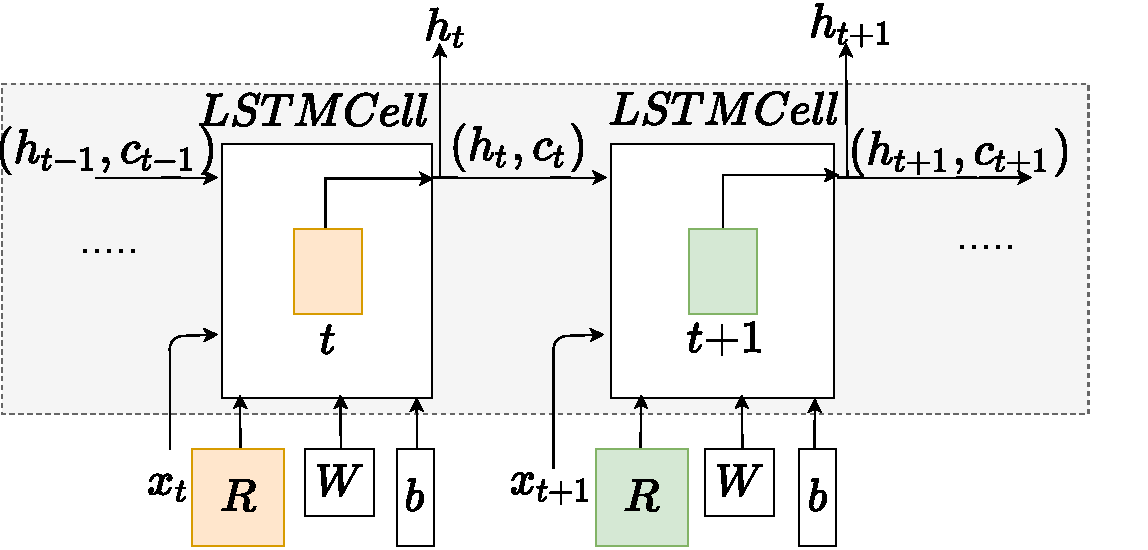
\includegraphics[width=0.4\textwidth]{introA.pdf}
		\label{fig:introA}}
	\hfil
	\subfloat[Proposed approach: $R$ matrix accesses are reduced by half. ]
	{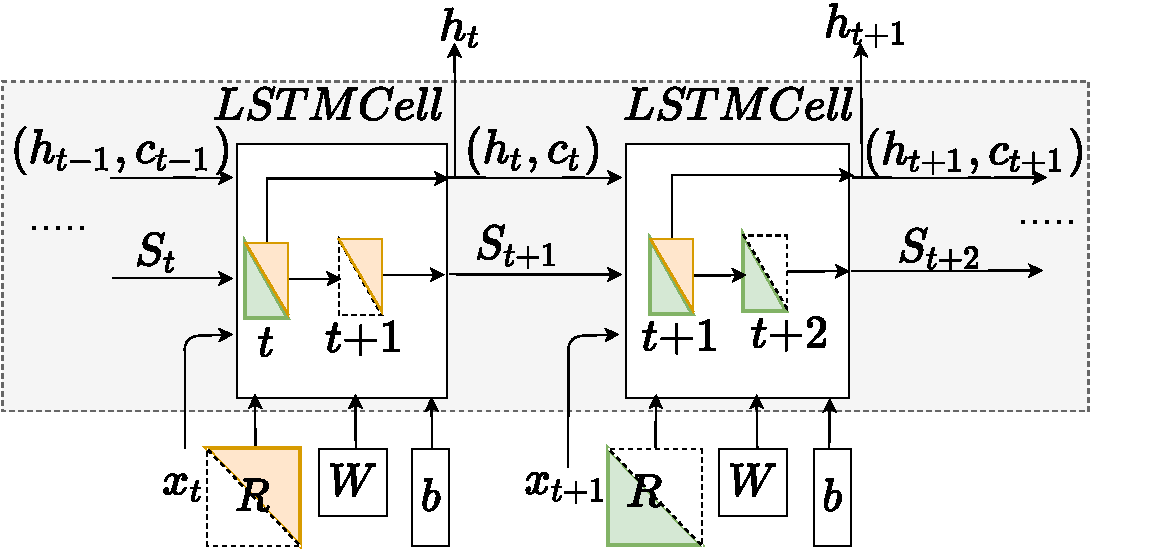
\includegraphics[width=.4\textwidth]{introB.pdf}
		\label{fig:introB}}
	\hfil	
	\caption{LSTM cell computations for consecutive time-steps showing the weight accesses.}
	\label{fig:introToApproach}
	\vspace{-1.0em}	
\end{figure}
\subsection{Proposed Approach}
We proposes an approach that reduces off-chip memory accesses by splitting the computation in two. At each time step, while the computations of a hidden state vector of one time step $h_t$ completes, partial computation of next time step ($S_{t+1}$) is also performed by reusing the weights.
Our approach schedules the computations in a way that reuses all the weights of $R$ between two adjacent time steps. The data reuse in our approach is independent of on-chip buffer sizes which makes it suitable for accelerators with very small on-chip memory.

The proposed data reuse approach splits and combines the LSTM cell computations in a way that reduces the off-chip memory accesses of hidden state matrices by 50\%. The computation of the $h_t$ can be expressed as shown below
\begin{align}\label{eq:h_{t}}
	h_{t}[k] &= F( S_{t}[k]+q_{t}[k])
\end{align}
where $F$ is a non-linear function. $q_{t}$ is computed as $W{\cdot}x_t{+}b$ and its computations are independent of previous step cell states. $S_{t}[k]$ is the sum of $N$ product terms as shown below,
\begin{align}
	S_{t}[k] = \sum_{n=0}^{N-1}R[k][n]\cdot h_{t-1}[n]
\end{align}
$S_{t}[k]$ can be computed as a sum of the following two partial sums $S_{t}^{L}[k]$ and $S_{t}^{U}[k]$
\begin{align}      
	S_{t}^{L}[k] &= \sum_{n=0}^{k}R[k][n]\cdot h_{t-1}[n] \label{eq:S_L_{t}}\\
	S_{t}^{U}[k] &= \sum_{n=k+1}^{N-1}R[k][n]\cdot h_{t-1}[n] \label{eq:S_U_{t}}
\end{align}
Equation~\eqref{eq:S_L_{t}} uses the lower-diagonal and diagonal elements of $R$ ($R^L$), and~\eqref{eq:S_U_{t}} uses the upper diagonal elements of $R$ ($R^U$). 
\begin{figure}[!tb]
	\centerline{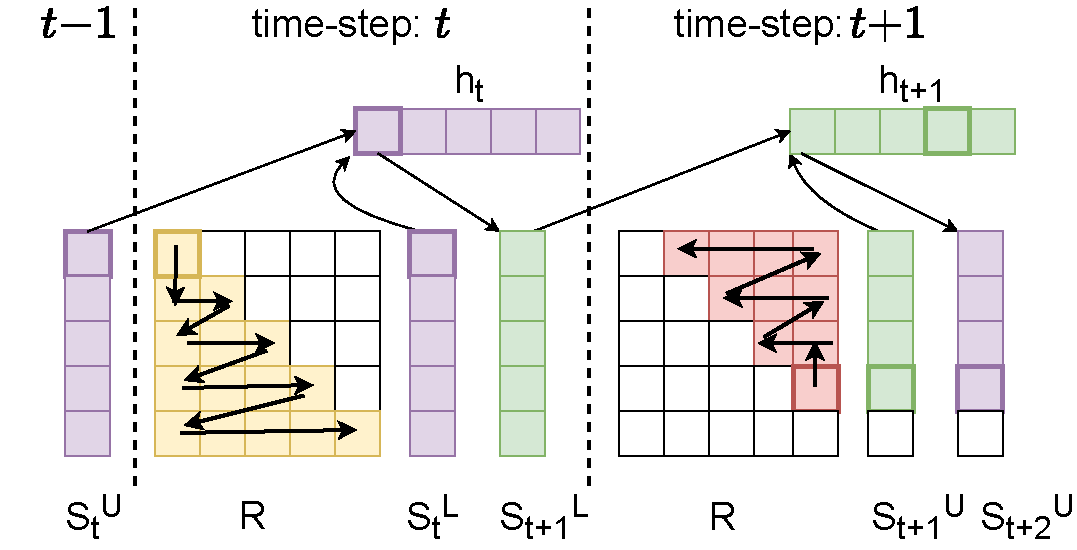
\includegraphics[width=0.5\textwidth]{TwoTimeSteps.pdf}}
	\caption{Splitting the hidden state vector computations into partial sums}
	\label{fig:TwoTimeStepsComputation}
	\vspace{-1.0em}	
\end{figure}
As shown in \figurename{~\ref{fig:TwoTimeStepsComputation}}, $R^L$ and $R^U$ are accessed in consecutive time steps and reused in the partial sum computations of two steps. At time step $t$, $S_t^U$ and $h_{t-1}$ are the inputs from the previous time step, and $R^L$ is reused to compute the partial sums $S_{t}^{L}$ and $S_{t+1}^L$. Input $S_{t}^{U}$ is added to $S_{t}^{L}$ to compute $h_{t}$, and $S_{t+1}^L$ is passed to $(t{+}1)^{th}$ step computations.
In the same way, at time step $t{+}1$, $R^U$ is reused to compute $S_{t+1}^{U}$ and $S_{t+2}^{U}$. Elements of $R^L$ are accessed from top to bottom, left to right, while elements of $R^U$ are accessed in the reverse order to satisfy the dependencies. As shown in~\figurename{~\ref{fig:TwoTimeStepsComputation}}, the proposed approach accesses the weight matrix $R$ once, to compute $h_{t}$ and $h_{t+1}$. 
%\footnotesize
\bibliographystyle{abbrv} %IEEEtran % abbrv
%\vspace{1.5mm}
\bibliography{refs}
%\nocite{*}
%\end{spacing}

\end{document}
